% !TeX root = RJwrapper.tex
\title{SurveyNCD: Design-Based Multimorbidity, Health-Inequality and Child-Growth Indicators from Complex Population Surveys}
\author{by Sujon Mia}

\maketitle

\abstract{%
Population health surveys such as the WHO STEPS surveys, the Demographic and Health Surveys and the Multiple Indicator Cluster Surveys record chronic conditions as self-reported answers and select respondents by stratified, clustered, unequal-probability designs. Turning those answers into defensible population estimates involves recoding inconsistent response codes, handling ``don't know'' answers, and carrying the design through to every standard error. The \CRANpkg{SurveyNCD} package provides small, tested functions for this workflow: binary recoding, a self-reported multimorbidity count, design-based prevalence, a survey-weighted concentration index with design-based standard errors, categorisation of DHS-coded child growth z-scores, choropleth mapping and an exploratory weighted gradient-boosting module. We illustrate every function on simulated data drawn from a known population, validate the concentration index against \CRANpkg{rineq} and a design bootstrap, and show in a 1,000-sample simulation that full-design intervals reach close to nominal coverage while analyses that ignore clustering do not.
}

\section{Introduction}

Multimorbidity, the presence of two or more chronic conditions in one person, is common and rising, and it is socially patterned \citep{barnett2012, afshar2015}. In low- and middle-income countries much of what is known about it comes from household surveys: the WHO STEPwise approach to non-communicable disease risk-factor surveillance \citep[STEPS;][]{riley2016}, the Demographic and Health Surveys \citep[DHS;][]{corsi2012} and the Multiple Indicator Cluster Surveys \citep[MICS;][]{khan2019}. These surveys share two features that shape the analysis. First, conditions are recorded as answers to questions such as ``Has a doctor or health worker ever told you that you have high blood pressure?'', coded in instrument-specific ways (1 = yes, 2 = no, 9 = don't know; or text). Second, respondents are selected by multi-stage designs with stratification, clustering and unequal selection probabilities, so that unweighted summaries are biased when the weights are informative and standard errors that ignore clustering are too small \citep{lumley2010}.

The \CRANpkg{survey} package \citep{lumley2004, lumley2010} provides the estimators these designs require. What it deliberately does not provide is the domain-specific layer that sits on top: deciding what a ``don't know'' does to a multimorbidity count, estimating subgroup prevalence without dropping rows from the design, ranking respondents by wealth for a concentration index when many share the same value, and decoding DHS conventions for anthropometric z-scores. In practice this layer is rewritten by hand for each project, and the mistakes it invites (missing answers counted as ``no condition'', subgroups analysed by subsetting the data frame, clustering ignored) leave no visible trace in the output.

\CRANpkg{SurveyNCD} packages that layer as ten exported functions built on \CRANpkg{survey}. This article describes the methods they implement and the design choices behind them, demonstrates every function on simulated data shipped with the package, and reports three kinds of validation: agreement with an independent implementation, robustness to the order of the data, and the frequency properties of the estimators over repeated samples from a known population.

\section{Methods implemented}

\subsection{Design-based estimation}

Let unit $k$ in stratum $h$ and primary sampling unit (PSU) $c$ have sampling weight $w_{hck}$, the inverse of its inclusion probability. The prevalence of a binary indicator $y$ is estimated by the ratio
\begin{equation}
\hat p = \frac{\sum_{h,c,k} w_{hck}\, y_{hck}}{\sum_{h,c,k} w_{hck}},
\label{eq:ratio}
\end{equation}
and its variance by Taylor linearisation with the with-replacement approximation at the first stage \citep{binder1983, lumley2010}. Confidence intervals for proportions are computed on the logit scale by \code{survey::svyciprop(method = "logit")}, which keeps them inside $[0, 1]$. Subgroup (domain) estimates are obtained with \code{subset()} applied to the design object, which keeps all PSUs in the variance calculation; subsetting the data frame before building the design is a common error that understates the variance.

\subsection{Self-reported multimorbidity}

Given binary condition indicators $c_{i1}, \dots, c_{iJ}$, the multimorbidity score is the weighted sum $\sum_j \omega_j c_{ij}$ with $\omega_j = 1$ by default, which is how the Functional Comorbidity Index \citep[FCI;][]{groll2005} is scored. The FCI was developed for self-reported conditions; \code{fci\_items()} returns its 18 conditions as a reference list. A respondent is classified as multimorbid when the unweighted count is at least two, the most common definition in prevalence studies \citep{fortin2012}. When fewer than the 18 FCI conditions are available, the score is a condition count rather than the validated FCI, and the documentation says so.

\subsection{Survey-weighted concentration index}

The concentration index measures how a health variable $y$ is distributed across the socioeconomic ranking \citep{wagstaff1991, odonnell2008}:
\begin{equation}
C = \frac{2}{\mu}\, \mathrm{cov}_w(y_i, R_i),
\label{eq:ci}
\end{equation}
where $\mu$ is the weighted mean of $y$ and $R_i$ the weighted fractional rank. For respondents sorted by wealth with cumulative weight $W_i = \sum_{j \le i} w_j$ and total $W$, the fractional rank is the mid-point of each respondent's interval of the cumulative distribution, $R_i = (W_{i-1} + w_i/2)/W$ \citep{lerman1989}. When respondents are tied on the ranking variable, which is unavoidable with wealth quintiles, sorting places them in an arbitrary order and this formula then gives tied respondents different ranks. \pkg{SurveyNCD} instead assigns every member of a tied group $g$ occupying the cumulative-weight interval $[L_g, U_g]$ the common rank $R_i = (L_g + U_g)/(2W)$, so the estimate depends only on the data and not on their order.

The point estimate and its standard error are obtained from the convenient regression of \citet{kakwani1997},
\begin{equation}
2\sigma_R^2 \frac{y_i}{\mu} = \alpha + \beta R_i + \varepsilon_i ,
\label{eq:convreg}
\end{equation}
where $\sigma_R^2$ is the weighted variance of $R_i$ and $\hat\beta = C$. Fitting Equation~\ref{eq:convreg} with \code{survey::svyglm()} gives a design-based sandwich standard error \citep{lumley2017}. This standard error treats the ranks and $\mu$ as fixed; we assess the consequence of that simplification against a bootstrap that recomputes them (Section~\nameref{sec:validation}).

\subsection{Child anthropometry}

DHS recode files store height-for-age, weight-for-age and weight-for-height z-scores multiplied by 100 (variables \code{hw70}, \code{hw71}, \code{hw72}) and use codes 9996--9999 for flagged or missing measurements. \code{who\_anthro\_score()} rescales the values, sets the codes to missing, removes biologically implausible values using the WHO limits (height-for-age outside $\pm 6$; weight-for-height outside $\pm 5$; weight-for-age below $-6$ or above $5$) and classifies the result as severe ($< -3$), moderate ($-3$ to $< -2$) or normal \citep{who2006}. It does not compute z-scores from raw measurements; for that, the WHO \CRANpkg{anthro} package is the reference implementation.

\section{Related software}

Table~\ref{tab:related} positions \pkg{SurveyNCD} among related R packages. Comorbidity packages such as \CRANpkg{comorbidity} \citep{gasparini2018} and \CRANpkg{multimorbidity} \citep{bensken2023} map ICD-9 and ICD-10 diagnosis codes in claims or clinical records to Charlson, Elixhauser and related scores; they do not apply to self-reported survey answers and do not estimate population quantities. \CRANpkg{rineq} \citep{rineq} computes relative, generalised and Erreygers-corrected \citep{erreygers2009} concentration indices with decomposition, using weights for the point estimate and an independence-based variance. \CRANpkg{healthequal} \citep{healthequal} computes 21 summary measures of inequality from disaggregated subgroup estimates. \CRANpkg{anthro} \citep{anthro} computes WHO growth-standard z-scores and design-based prevalence from raw measurements. \pkg{SurveyNCD} overlaps with each of these at one point. Its contribution is to connect self-reported multimorbidity scoring, domain prevalence and a design-based concentration index in one workflow on \pkg{survey} design objects, not to provide new estimators.

\begin{table}[htbp]
\centering\small
\caption{\label{tab:related}Scope of \pkg{SurveyNCD} and related R packages (as described in each package's documentation).}
\begin{tabular}{p{2.3cm}p{3.6cm}p{2.6cm}p{4.2cm}}
\toprule
Package & Main input & Design-based SEs & Focus \\
\midrule
\pkg{survey} & Respondent microdata & Yes & General estimators for complex designs \\
\pkg{comorbidity} & ICD-coded diagnoses & No & Charlson/Elixhauser scores \\
\pkg{multimorbidity} & ICD-coded claims & No & Comorbidity, multimorbidity and frailty measures \\
\pkg{rineq} & Respondent microdata & No (weights in point estimate) & Concentration indices and decomposition \\
\pkg{healthequal} & Subgroup estimates & From input estimates & 21 summary measures of inequality \\
\pkg{anthro} & Raw child measurements & Yes & WHO z-scores and prevalence \\
\pkg{SurveyNCD} & Respondent microdata, raw codes & Yes & Self-reported multimorbidity, domain prevalence, design-based concentration index \\
\bottomrule
\end{tabular}
\end{table}

\section{Package design}

Figure~\ref{fig:workflow} shows how the ten functions fit together. Four decisions shape the package.

\begin{figure}[htbp]
\centering
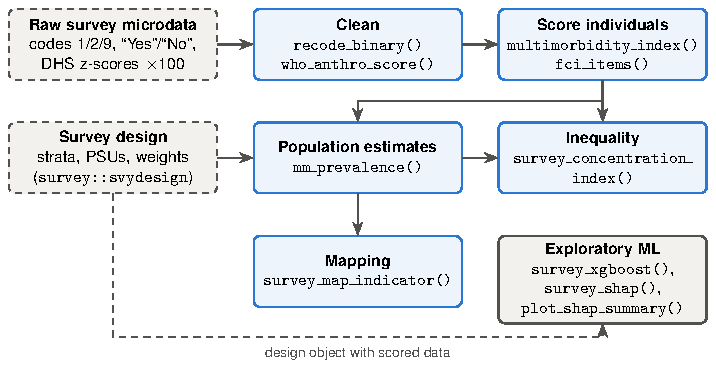
\includegraphics[width=\linewidth,alt={Flow diagram: raw survey microdata are cleaned with recode_binary and who_anthro_score, scored with multimorbidity_index, combined with the survey design in mm_prevalence, then passed to survey_concentration_index, survey_map_indicator and the exploratory machine-learning functions.}]{figures/fig_workflow}
\caption{\label{fig:workflow}Workflow of \pkg{SurveyNCD}. Solid boxes are package functions; dashed boxes are inputs. Exploratory machine learning is shaded to mark that it does not provide design-based inference.}
\end{figure}

\emph{A thin layer over \pkg{survey}.} All variance estimation is delegated to \code{svydesign()}, \code{svyciprop()}, \code{svymean()} and \code{svyglm()}. \code{mm\_prevalence()} accepts column names and builds the design internally, while \code{survey\_concentration\_index()} accepts any \code{survey.design} object, including those made by \CRANpkg{srvyr}. Both set \code{options(survey.lonely.psu = "adjust")} for the duration of the call, because single-PSU strata arise easily in subgroup analyses, and restore the user's setting on exit.

\emph{Missing answers are a stated policy.} \code{recode\_binary()} warns about any value it cannot place instead of guessing. \code{multimorbidity\_index()} takes \code{na\_action = "na"} (any missing condition gives a missing score) or \code{"ignore"} (sum the answered conditions); under either policy a respondent with every condition missing is scored as missing, never as healthy. \code{mm\_prevalence()} reports how many respondents it excluded.

\emph{Results do not depend on the order of the data.} This is the reason for the tie rule for fractional ranks described above.

\emph{Exploratory methods are fenced off.} \code{survey\_xgboost()} passes the sampling weights to \CRANpkg{xgboost} \citep{chen2016} as case weights; \code{survey\_shap()} extracts SHAP attributions \citep{lundberg2017} and \code{plot\_shap\_summary()} plots them. Strata and clusters play no part in any of these, so the documentation describes them as exploratory. \pkg{xgboost} and \CRANpkg{sf} \citep{pebesma2018} are suggested rather than imported.

\section{Example data}

The package ships two simulated datasets so that every function can be run immediately. They are drawn from a synthetic population whose generating code is in \file{data-raw/} of the source repository. Because the population is known, estimates can be compared with the truth.

The population has six regions of unequal size (60 to 300 enumeration areas each, 950 in total), each divided into urban and rural areas, giving 12 strata. It contains 142,133 households with one adult aged 18--69 each, and 64,169 children under five. Each adult's seven conditions are drawn from logistic models in age, sex, body mass index, household wealth and an area-level random effect. The wealth gradient is positive for hypertension and diabetes and negative for arthritis, asthma and depression. Child z-scores depend on wealth, age and an area effect. The sample selects ten areas by simple random sampling in every stratum and 20 households in each, so small regions and urban areas are over-sampled. Inclusion probabilities are exact, giving the design weights; these vary 15-fold (Table~\ref{tab:tab_dataset}). Condition answers are coded as in STEPS with 1--4\% ``don't know'' per item, and child z-scores follow DHS coding with flag codes and a few implausible values.

\begin{table}[htbp]

\caption{\label{tab:tab_dataset}The simulated example datasets shipped with SurveyNCD.}
\centering
\small
\begin{adjustbox}{max width=\linewidth}
\begin{tabular}{lr}
\toprule
Item & Value\\
\midrule
Adults (households) & 2400\\
Children under 5 & 1034\\
Strata & 12\\
Primary sampling units & 120\\
Weight range (normalised) & 0.21 to 3.08\\
Adults with any 'don't know' answer & 346 (14.4\%)\\
\bottomrule
\end{tabular}
\end{adjustbox}
\end{table}


\section{A worked analysis}

All results in this section come from \file{analysis/01\_worked\_example.R} in the repository. The code shown is abbreviated; the script runs in about ten seconds.

\subsection{Cleaning and scoring}

\begin{example}
library("SurveyNCD")
library("survey")
options(survey.lonely.psu = "adjust")
d <- ncd_survey
d$htn <- recode_binary(d$htn_raw, yes = 1, no = 2)
d$dep <- recode_binary(d$dep_raw, yes = "Yes", no = "No")
table(raw = d$dep_raw, clean = d$dep, useNA = "ifany")
#>             clean
#> raw             0    1 <NA>
#>   Don't know    0    0   72
#>   No         2176    0    0
#>   Yes           0  152    0
\end{example}

After recoding the other five items the same way, \code{multimorbidity\_index()} scores each respondent:

\begin{example}
conds <- c("htn", "dm", "arth", "asthma", "angina", "stroke", "dep")
scored <- multimorbidity_index(d, conditions = conds, na_action = "na")
table(scored$mm_category, useNA = "ifany")
#>             None Single condition      Multimorbid             <NA>
#>             1310              557              187              346
\end{example}

The 346 respondents (14.4\%) with at least one ``don't know'' receive a missing score instead of being counted as free of that condition.

\subsection{Prevalence}

Table~\ref{tab:tab_condition_prevalence} compares design-based estimates for each condition with unweighted sample percentages and with the true population values. Design effects of 1.1 to 2.7 show how much clustering inflates the variance relative to simple random sampling.

\begin{table}[htbp]

\caption{\label{tab:tab_condition_prevalence}Self-reported prevalence of each condition in the simulated survey: design-based estimates (strata, clusters, weights; logit 95\% CI), unweighted sample percentages, the true value in the simulated population, and the design effect.}
\centering
\small
\begin{adjustbox}{max width=\linewidth}
\begin{tabular}{lrrrrr}
\toprule
Condition & Don't know (n) & Design-based \% (95\% CI) & Unweighted \% & Population truth \% & Design effect\\
\midrule
Hypertension & 92 & 17.0 (14.8, 19.5) & 16.5 & 15.8 & 2.36\\
Diabetes & 68 & 7.1 (5.6, 9.1) & 6.8 & 7.4 & 2.69\\
Arthritis & 38 & 10.4 (9.0, 12.0) & 9.9 & 10.1 & 1.47\\
Asthma & 12 & 3.9 (3.1, 4.9) & 4.0 & 4.1 & 1.27\\
Angina / heart disease & 53 & 3.1 (2.2, 4.3) & 3.0 & 3.2 & 1.98\\
Stroke & 34 & 0.8 (0.5, 1.3) & 1.1 & 1.2 & 1.09\\
Depression & 72 & 6.5 (5.2, 8.1) & 6.5 & 6.0 & 1.98\\
\bottomrule
\end{tabular}
\end{adjustbox}
\end{table}


\begin{example}
mm_prevalence(scored, ids = "psu", strata = "stratum", weights = "wt")
#> 346 of 2400 rows have a missing multimorbidity score and are excluded
#> from the survey-weighted estimate.
#>      n prevalence prevalence_se prevalence_lower prevalence_upper
#> 1 2054 0.09533923    0.01175125       0.07445529        0.1213131
#>   mean_conditions mean_conditions_se
#> 1       0.4850582         0.02954051
\end{example}

The design-based multimorbidity prevalence of 9.5\% (95\% CI 7.4--12.1\%) matches the population value of 9.49\%; the unweighted sample proportion is 9.1\%. Subgroup estimates use the \code{by} argument (Table~\ref{tab:tab_multimorbidity}). Figure~\ref{fig:mm} shows them by wealth quintile and residence. With 2,000 respondents the intervals are wide and the gradient in multimorbidity is not monotone, which is consistent with the simulated population, where conditions with opposite wealth gradients largely cancel in the count.

\begin{table}[htbp]

\caption{\label{tab:tab_multimorbidity}Design-based prevalence of multimorbidity (two or more of seven self-reported conditions) and mean number of conditions, from mm\_prevalence(). 346 of 2400 respondents with any `don't know' answer were excluded. True population values: multimorbidity 9.5\%, mean 0.48 conditions.}
\centering
\small
\begin{adjustbox}{max width=\linewidth}
\begin{tabular}{llrrr}
\toprule
Characteristic & Group & n & Multimorbidity \% (95\% CI) & Mean conditions (SE)\\
\midrule
All adults &  & 2054 & 9.5 (7.4, 12.1) & 0.49 (0.030)\\
Sex & Female & 1050 & 9.9 (7.4, 13.2) & 0.50 (0.037)\\
 & Male & 1004 & 9.1 (6.8, 12.2) & 0.47 (0.036)\\
Residence & Rural & 1038 & 9.3 (6.6, 12.9) & 0.48 (0.038)\\
 & Urban & 1016 & 10.1 (7.5, 13.5) & 0.49 (0.044)\\
Wealth quintile & Q1 (poorest) & 399 & 8.5 (5.0, 13.9) & 0.46 (0.054)\\
 & Q2 & 418 & 9.4 (6.1, 14.1) & 0.48 (0.044)\\
 & Q3 & 404 & 11.9 (7.6, 18.3) & 0.52 (0.061)\\
 & Q4 & 396 & 5.9 (3.7, 9.4) & 0.42 (0.039)\\
 & Q5 (richest) & 437 & 11.9 (8.2, 17.1) & 0.55 (0.051)\\
Region & Region A & 341 & 10.1 (6.6, 15.2) & 0.48 (0.054)\\
 & Region B & 343 & 10.2 (4.7, 20.7) & 0.49 (0.091)\\
 & Region C & 342 & 10.6 (6.6, 16.6) & 0.56 (0.042)\\
 & Region D & 343 & 4.2 (2.3, 7.7) & 0.35 (0.037)\\
 & Region E & 336 & 10.5 (6.4, 16.7) & 0.51 (0.074)\\
 & Region F & 349 & 10.9 (7.0, 16.4) & 0.55 (0.059)\\
\bottomrule
\end{tabular}
\end{adjustbox}
\end{table}


\begin{figure}[htbp]
\centering
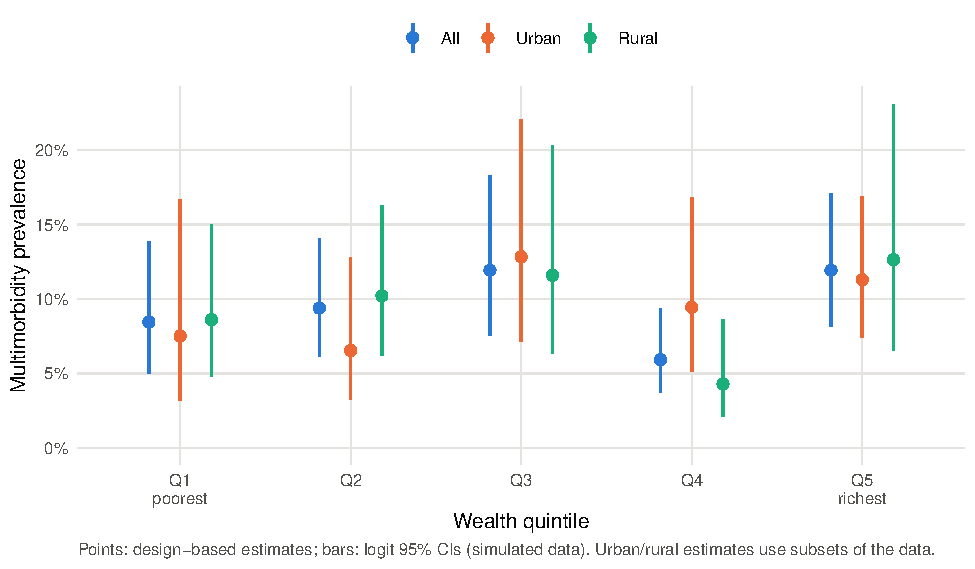
\includegraphics[width=\linewidth,alt={Dot-and-interval plot of multimorbidity prevalence by wealth quintile for all adults, urban and rural; estimates range from about 4 to 13 percent with wide overlapping intervals.}]{figures/fig_mm_by_wealth}
\caption{\label{fig:mm}Design-based multimorbidity prevalence by wealth quintile, overall and by residence, with logit 95\% confidence intervals (simulated data).}
\end{figure}

\subsection{Inequality}

\begin{example}
des <- svydesign(ids = ~psu, strata = ~stratum, weights = ~wt,
                 data = scored, nest = TRUE)
survey_concentration_index(des, outcome = dm, wealth = wealth_score)
#> # A tibble: 1 x 7
#>   Concentration_Index Standard_Error Lower_CI Upper_CI  p_value Outcome_Mean
#>                 <dbl>          <dbl>    <dbl>    <dbl>    <dbl>        <dbl>
#> 1               0.314         0.0547    0.206    0.421  1.00e-8       0.0714
#> # i 1 more variable: n <int>
\end{example}

Table~\ref{tab:tab_concentration_indices} and Figure~\ref{fig:ci} report concentration indices for each condition, the condition count, multimorbidity and child undernutrition. Diabetes and hypertension are concentrated among richer adults and depression among poorer adults, as built into the simulation. Because these gradients cancel, the concentration index for the condition count is close to zero (true value 0.028), which illustrates that a count can hide opposing inequalities in its components.

\begin{table}[htbp]

\caption{\label{tab:tab_concentration_indices}Wealth-related concentration indices from survey\_concentration\_index() (ranking: continuous wealth score). Negative values: concentrated among poorer people; positive: among richer people. Design-based SEs account for strata and clusters.}
\centering
\small
\begin{adjustbox}{max width=\linewidth}
\begin{tabular}{llrrrr}
\toprule
Outcome & Population & CI (95\% CI) & SE & p & n\\
\midrule
Hypertension & Adults & 0.123 (0.065, 0.181) & 0.030 & <0.001 & 2308\\
Diabetes & Adults & 0.314 (0.206, 0.421) & 0.055 & <0.001 & 2332\\
Arthritis & Adults & -0.083 (-0.168, 0.001) & 0.043 & 0.052 & 2362\\
Asthma & Adults & -0.057 (-0.189, 0.076) & 0.068 & 0.401 & 2388\\
Angina / heart disease & Adults & 0.019 (-0.129, 0.166) & 0.075 & 0.805 & 2347\\
Stroke & Adults & -0.199 (-0.503, 0.104) & 0.155 & 0.198 & 2366\\
Depression & Adults & -0.153 (-0.266, -0.040) & 0.058 & 0.008 & 2328\\
Number of conditions & Adults & 0.025 (-0.028, 0.079) & 0.027 & 0.352 & 2054\\
Multimorbidity & Adults & 0.036 (-0.070, 0.142) & 0.054 & 0.502 & 2054\\
Stunting & Children & -0.250 (-0.312, -0.188) & 0.032 & <0.001 & 1015\\
Underweight & Children & -0.342 (-0.432, -0.252) & 0.046 & <0.001 & 1009\\
Wasting & Children & -0.210 (-0.374, -0.046) & 0.084 & 0.012 & 1007\\
\bottomrule
\end{tabular}
\end{adjustbox}
\end{table}


\begin{figure}[htbp]
\centering
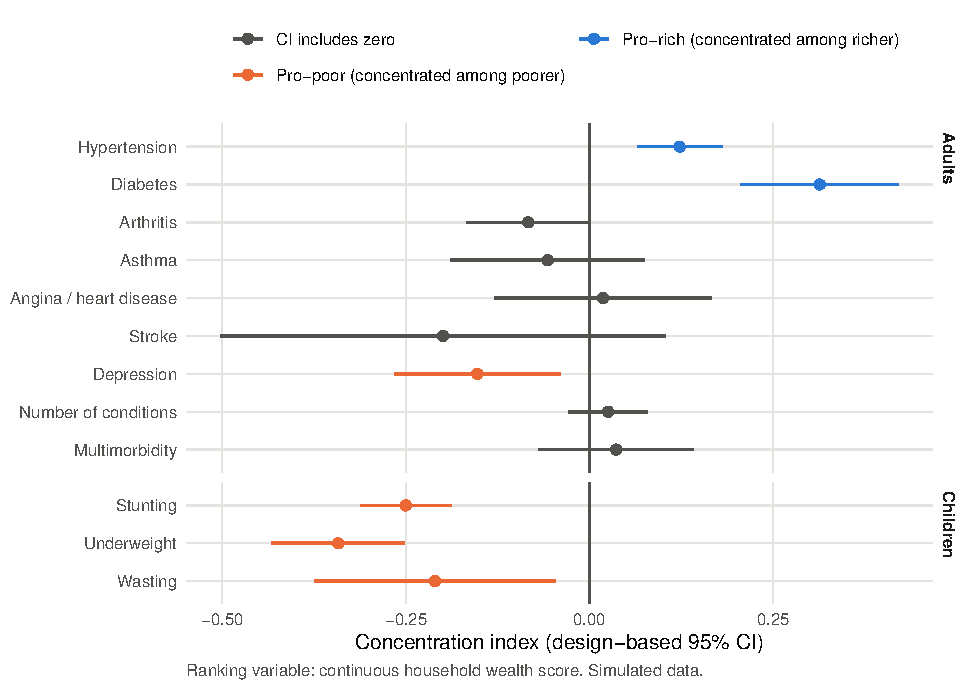
\includegraphics[width=0.92\linewidth,alt={Forest plot of concentration indices: hypertension and diabetes positive (pro-rich), depression and child stunting, underweight and wasting negative (pro-poor), others include zero.}]{figures/fig_concentration_indices}
\caption{\label{fig:ci}Wealth-related concentration indices with design-based 95\% confidence intervals (simulated data). Colour marks the direction when the interval excludes zero.}
\end{figure}

\subsection{Child undernutrition}

\begin{example}
ch <- child_anthro
ch$stunting <- who_anthro_score(ch$hw70, indicator = "stunting")
table(ch$stunting, useNA = "ifany")
#>   Severe stunting Moderate stunting   Normal stunting              <NA>
#>                81               209               725                19
\end{example}

Table~\ref{tab:tab_anthropometry} summarises the three indicators after flag codes and implausible values are removed. In this particular sample the stunting interval (26.9--34.1\%) narrowly misses the population value of 26.8\%. That is the kind of event a 95\% interval should produce about once in twenty samples, and the simulation study below shows its long-run coverage. Stunting is strongly concentrated among poorer children ($C = -0.250$, 95\% CI $-0.312$ to $-0.188$; population value $-0.259$).

\begin{table}[htbp]

\caption{\label{tab:tab_anthropometry}Child undernutrition from DHS-coded z-scores using who\_anthro\_score(): flag codes and biologically implausible values set to missing, then design-based prevalence.}
\centering
\footnotesize\setlength{\tabcolsep}{3pt}
\begin{adjustbox}{max width=\linewidth}
\begin{tabular}{lrrrrrr}
\toprule
Indicator & DHS flag codes (n) & Implausible removed (n) & Analysed (n) & Severe \% & Moderate \% & Moderate or severe \% (95\% CI)\\
\midrule
Stunting (HAZ < -2) & 12 & 7 & 1015 & 8.9 & 21.5 & 30.4 (26.9, 34.1)\\
Underweight (WAZ < -2) & 19 & 6 & 1009 & 4.0 & 14.2 & 18.2 (14.7, 22.3)\\
Wasting (WHZ < -2) & 21 & 6 & 1007 & 0.7 & 6.8 & 7.5 (5.8, 9.7)\\
\bottomrule
\end{tabular}
\end{adjustbox}
\end{table}


\subsection{Mapping and exploratory modelling}

Regional estimates from \code{mm\_prevalence(by = "region")} are joined to an \pkg{sf} object and drawn by \code{survey\_map\_indicator()} (Figure~\ref{fig:map}). Because the regions are fictitious, the example uses a schematic grid of six polygons; with real data, any boundary file with a matching key column works.

\begin{figure}[htbp]
\centering
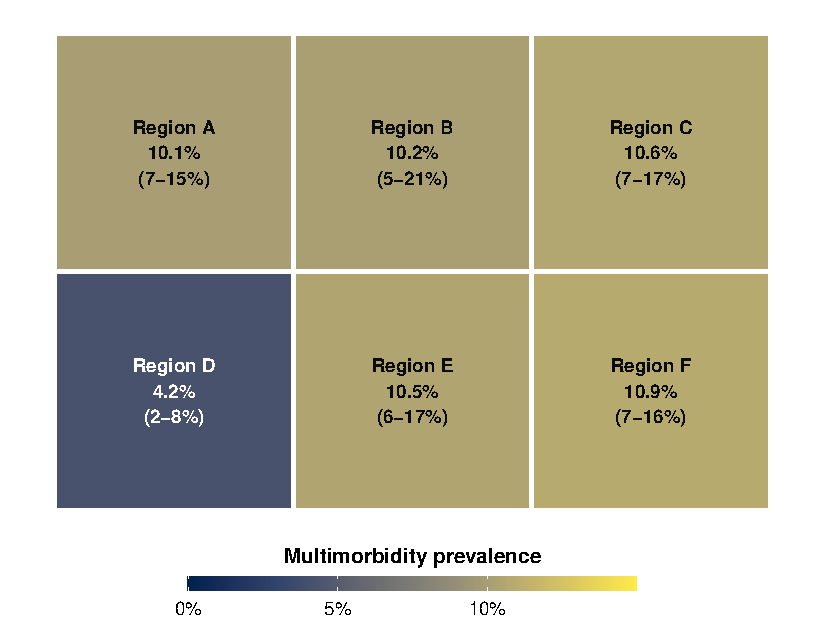
\includegraphics[width=0.72\linewidth,alt={Choropleth of six rectangular fictitious regions; Region D about 4 percent, the others about 10 to 11 percent.}]{figures/fig_region_map}
\caption{\label{fig:map}Multimorbidity prevalence by region, drawn with \code{survey\_map\_indicator()} on a schematic map of six fictitious regions. Labels give estimates and 95\% confidence intervals.}
\end{figure}

Finally, a weighted gradient-boosting model for the number of conditions with age, BMI, wealth, sex and residence as features ranks age as by far the most influential feature (mean absolute SHAP value 0.21), followed by BMI (0.08) and wealth (0.07); Figure~\ref{fig:shap}. These attributions describe the fitted model, not causal effects, and carry no design-based uncertainty.

\begin{figure}[htbp]
\centering
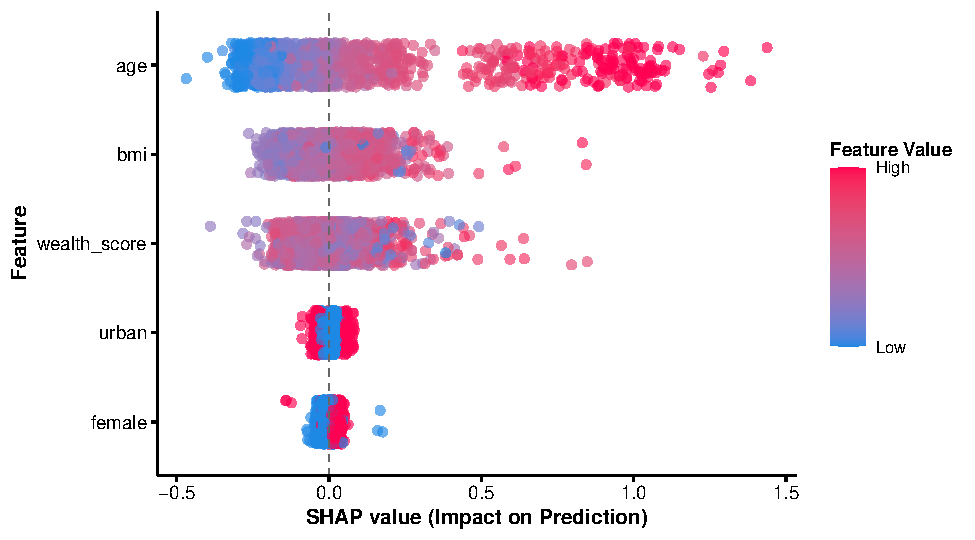
\includegraphics[width=0.9\linewidth,alt={SHAP summary plot; age has the widest spread of SHAP values, followed by BMI and wealth score; sex and residence contribute little.}]{figures/fig_shap_summary}
\caption{\label{fig:shap}SHAP summary for a survey-weighted gradient-boosting model of the number of conditions (\code{survey\_xgboost()}, \code{survey\_shap()}, \code{plot\_shap\_summary()}; 300 rounds, depth 3). Exploratory: case weights only.}
\end{figure}

\section{Validation}
\label{sec:validation}

\subsection{Agreement with an independent implementation}

Table~\ref{tab:tab_validation_rineq} compares \code{survey\_concentration\_index()} with \code{rineq::ci()} on the same weighted data. The wealth score is recorded to three decimals and has tied values. \pkg{rineq} ranks ties by their position in the data while \pkg{SurveyNCD} gives them a common rank, so the two differ by up to $4\times10^{-5}$. With the ties broken by a negligible perturbation, they agree to within $5\times10^{-16}$. For standard errors, the design-based value from \pkg{SurveyNCD} is within 11\% of a 500-replicate bootstrap that resamples PSUs within strata and recomputes the ranks and the mean in every replicate. This supports treating the ranks as fixed in Equation~\ref{eq:convreg} at this sample size. The independence-based standard error from \pkg{rineq} is 9--27\% smaller, as expected when clustering is ignored.

\begin{table}[htbp]

\caption{\label{tab:tab_validation_rineq}Concentration index (adults with complete answers on all seven conditions, n = 2054) from survey\_concentration\_index() compared with rineq::ci() (version 0.0.2) and with a 500-replicate design bootstrap that re-computes the fractional ranks in every replicate. The wealth score has 379 tied values; rineq ranks ties by row order while SurveyNCD gives tied respondents a common mid-rank, which explains the small differences; with ties broken the two agree to rounding error. rineq's standard error assumes independent observations and ignores strata and clusters.}
\centering
\scriptsize\setlength{\tabcolsep}{3pt}
\begin{adjustbox}{max width=\linewidth}
\begin{tabular}{lrrrrrrr}
\toprule
Outcome & SurveyNCD CI & rineq CI & Abs. diff. (ties) & Abs. diff. (no ties) & SE: SurveyNCD (design) & SE: bootstrap (design) & SE: rineq (iid)\\
\midrule
Hypertension & 0.103 & 0.103 & 4.2e-05 & 3.5e-16 & 0.032 & 0.033 & 0.029\\
Diabetes & 0.320 & 0.320 & 1.9e-05 & 1.7e-16 & 0.060 & 0.056 & 0.044\\
Depression & -0.194 & -0.194 & 2.3e-05 & 4.2e-16 & 0.063 & 0.057 & 0.048\\
Number of conditions & 0.025 & 0.025 & 2.4e-05 & 9.4e-17 & 0.027 & 0.026 & 0.020\\
Multimorbidity & 0.036 & 0.036 & 3.9e-05 & 6.9e-18 & 0.054 & 0.052 & 0.040\\
\bottomrule
\end{tabular}
\end{adjustbox}
\end{table}


\subsection{Order invariance}

Version 0.1.0 of \pkg{SurveyNCD} assigned tied respondents ranks by row order. Table~\ref{tab:tab_validation_ties} reports the concentration index of the condition count ranked by wealth quintile over 50 random orderings of the same data. Under the old rule the estimate ranged from 0.011 to 0.029 around a reference value of 0.020, a spread almost as large as the estimate. The current rule returns 0.020 every time. A regression test guards this behaviour.

\begin{table}[htbp]

\caption{\label{tab:tab_validation_ties}Concentration index of the number of conditions ranked by wealth quintile (five tied groups), over 50 random row orders of the same data.}
\centering
\small
\begin{adjustbox}{max width=\linewidth}
\begin{tabular}{lrrrr}
\toprule
Version & Min CI & Max CI & Range & Reference (mid-rank)\\
\midrule
0.1.0 (row-order ranks) & 0.011 & 0.029 & 0.018 & 0.020\\
0.2.0 (mid-ranks for ties) & 0.020 & 0.020 & 5.1e-16 & 0.020\\
\bottomrule
\end{tabular}
\end{adjustbox}
\end{table}


\subsection{Simulation study}

To assess bias and interval coverage, we drew 1,000 independent samples from the population with the same design and analysed each in three ways: the full design (strata, PSUs, weights) as \pkg{SurveyNCD} does; weights only, ignoring strata and clusters; and an unweighted analysis assuming independent observations. Following \citet{morris2019}, Table~\ref{tab:tab_simulation} reports relative bias, the ratio of the mean estimated standard error to the empirical standard deviation of the estimates, and coverage of nominal 95\% intervals. The Monte Carlo standard error of coverage is about 0.7 percentage points.

\begin{table}[htbp]

\caption{\label{tab:tab_simulation}Monte Carlo evaluation over 1000 independent samples drawn with the same stratified two-stage design from one simulated population (142,133 adults; 64,169 children). Coverage of nominal 95\% intervals (Monte Carlo SE about 0.7 points). SE ratio = mean estimated SE / empirical SE.}
\centering
\scriptsize\setlength{\tabcolsep}{3pt}
\begin{adjustbox}{max width=\linewidth}
\begin{tabular}{llrrrrrrr}
\toprule
Estimand & Method & True value & Mean estimate & Rel. bias \% & Empirical SE & Mean model SE & SE ratio & Coverage \%\\
\midrule
Multimorbidity prevalence & Full design (SurveyNCD) & 0.0949 & 0.0953 & 0.4 & 0.0093 & 0.0094 & 1.01 & 95.5\\
 & Weights only &  & 0.0953 & 0.4 & 0.0093 & 0.0078 & 0.84 & 90.7\\
 & Unweighted, iid &  & 0.0959 & 1.1 & 0.0075 & 0.0065 & 0.87 & 90.5\\
CI: number of conditions & Full design (SurveyNCD) & 0.0275 & 0.0284 & 2.9 & 0.0261 & 0.0260 & 0.99 & 94.2\\
 & Weights only &  & 0.0284 & 2.9 & 0.0261 & 0.0236 & 0.90 & 92.6\\
 & Unweighted, iid &  & 0.0331 & 20.0 & 0.0223 & 0.0200 & 0.89 & 91.6\\
Stunting prevalence & Full design (SurveyNCD) & 0.2684 & 0.2676 & -0.3 & 0.0206 & 0.0199 & 0.97 & 93.4\\
 & Weights only &  & 0.2676 & -0.3 & 0.0206 & 0.0165 & 0.80 & 88.7\\
 & Unweighted, iid &  & 0.2642 & -1.6 & 0.0159 & 0.0135 & 0.85 & 88.9\\
CI: stunting & Full design (SurveyNCD) & -0.2589 & -0.2591 & -0.1 & 0.0349 & 0.0350 & 1.00 & 95.0\\
 & Weights only &  & -0.2591 & -0.1 & 0.0349 & 0.0333 & 0.95 & 93.9\\
 & Unweighted, iid &  & -0.2657 & -2.6 & 0.0288 & 0.0278 & 0.97 & 94.0\\
\bottomrule
\end{tabular}
\end{adjustbox}
\end{table}


\begin{figure}[htbp]
\centering
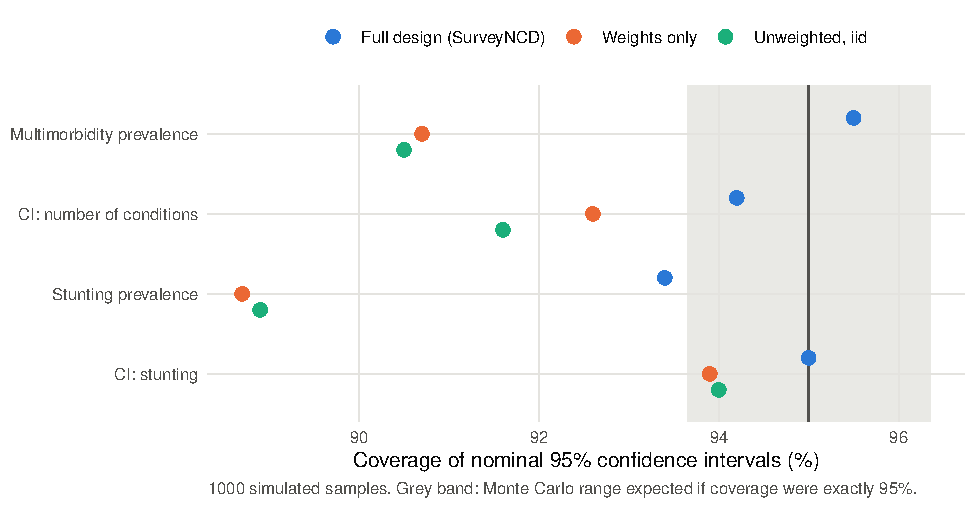
\includegraphics[width=0.9\linewidth,alt={Dot plot of 95 percent interval coverage for four estimands and three methods; full-design coverage lies near 95 percent, weights-only and unweighted methods fall to about 89 to 94 percent.}]{figures/fig_simulation_coverage}
\caption{\label{fig:sim}Coverage of nominal 95\% confidence intervals over 1,000 simulated samples. The grey band is the range expected from Monte Carlo error alone if coverage were exactly 95\%.}
\end{figure}

With the full design, bias was below 3\% for all four estimands, standard-error ratios were 0.97--1.01 and coverage was 93.4--95.5\% (Figure~\ref{fig:sim}). Ignoring strata and clusters left the point estimates unchanged but understated the standard errors by up to 20\%, and coverage fell to 88.7--93.9\%. The unweighted analysis also understated uncertainty and inflated the concentration index of the condition count by 20\%, because urban and small-region households were over-sampled. Full-design coverage for stunting prevalence (93.4\%) was slightly below nominal; with only ten PSUs per stratum, a $t$ reference distribution or a design-degrees-of-freedom correction would be a natural refinement.

The whole study takes about five minutes on one core (\file{analysis/03\_simulation\_study.R}).

\section{Limitations}

Complete-case exclusion under \code{na\_action = "na"} is unbiased only when ``don't know'' answers are missing completely at random; in the example it removed 14\% of respondents, and no weight adjustment is made. \code{mm\_prevalence()} and \code{survey\_concentration\_index()} take one grouping variable at a time. The concentration-index standard error treats ranks as fixed and uses a normal reference distribution. The validation above suggests this works at typical survey sizes, but it may not with few PSUs. \code{who\_anthro\_score()} covers undernutrition tiers only. The gradient-boosting module offers no design-based inference. The simulated population is a deliberately simple model and is not a substitute for validation against published estimates from real surveys, which we plan as the package is applied to STEPS and DHS microdata.

\section{Summary}

\pkg{SurveyNCD} turns raw self-reported survey answers into design-based estimates of multimorbidity, its socioeconomic distribution and child undernutrition, using \pkg{survey} for all variance estimation. Shipping simulated data with a known population, and the scripts that reproduce every table and figure here, lets users check what the functions do before applying them to their own surveys. The package is on CRAN, and development takes place at \url{https://github.com/StatAid-Research-Lab/SurveyNCD}.

\section{Acknowledgements}

The author thanks Professor Md. Atiqul Islam, Department of Statistics, Jagannath University, for academic mentorship. [TODO: funding statement, or ``No specific funding was received.'']

\emph{Use of generative AI.} [TODO, AUTHOR TO COMPLETE AND CONFIRM: Claude Sonnet 5.5 (Anthropic) was used to help write the package's R code. Claude (Anthropic) was used in October 2026 to help draft and edit this article and to write the simulation, validation and figure scripts. State the nature of the assistance with the code. Add the sentence that the author reviewed, ran and verified all code and results and takes responsibility for them, but only if this is true.]

\bibliography{mia}

\address{%
Sujon Mia\\
StatAid Research Lab\\
Department of Statistics, Jagannath University\\
Dhaka, Bangladesh\\
\textit{ORCID: \href{https://orcid.org/0009-0001-1032-2818}{0009-0001-1032-2818}}\\
\href{mailto:sujonsgc@gmail.com}{\nolinkurl{sujonsgc@gmail.com}}%
}
